\newpage
\section{Composite Pattern}

Composite pattern is used where we need to treat a group of objects in similar way as a single object. Composite pattern composes objects in term of a tree structure to represent part as well as whole hierarchy. This type of design pattern comes under structural pattern as this pattern creates a tree structure of group of objects.

This pattern creates a class that contains group of its own objects. This class provides ways to modify its group of same objects.

We are demonstrating use of composite pattern via following example in which we will show employees hierarchy of an organization.

\subsection{Implementation}

We have a class Employee which acts as composite pattern actor class. CompositePatternDemo, our demo class will use Employee class to add department level hierarchy and print all employees.

\subsection{Class Diagram}

\begin{figure}[h]
\centering
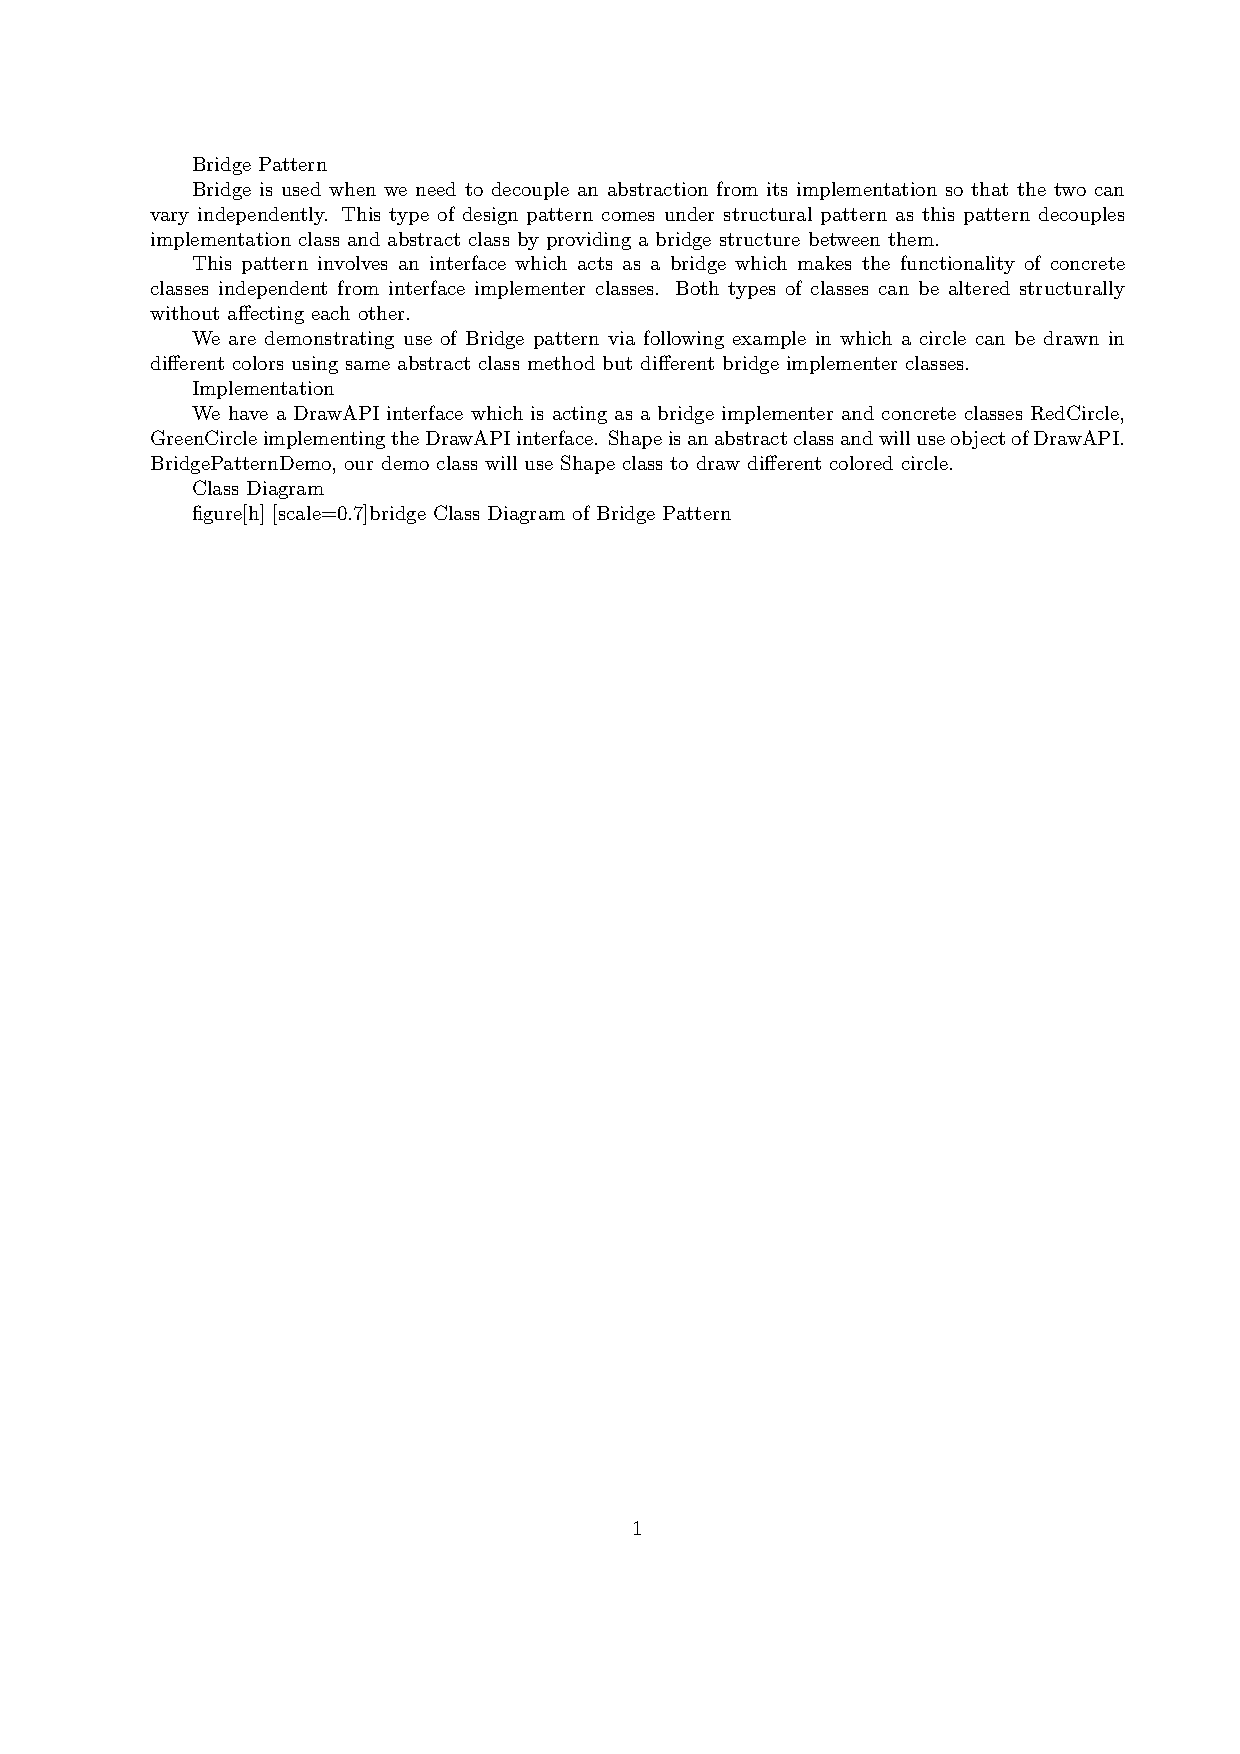
\includegraphics[scale=0.5]{composite}
\caption{Class Diagram of Composite Pattern}
\end{figure}

\newpage
\subsection{Source Code (Java)}

\subsubsection{Employee Class}

\begin{minted}{java}
import java.util.ArrayList;
import java.util.List;

public class Employee {
   private String name;
   private String dept;
   private int salary;
   private List<Employee> subordinates;

   // constructor
   public Employee(String name,String dept, int sal) {
      this.name = name;
      this.dept = dept;
      this.salary = sal;
      subordinates = new ArrayList<Employee>();
   }

   public void add(Employee e) {
      subordinates.add(e);
   }

   public void remove(Employee e) {
      subordinates.remove(e);
   }

   public List<Employee> getSubordinates(){
     return subordinates;
   }

   public String toString(){
      return ("Employee :[ Name : " + name + ", dept : " + dept + ", salary :" + salary+" ]");
   }   
}
\end{minted}

\subsubsection{Driver Class}

\begin{minted}{java}
public class CompositePatternDemo {
   public static void main(String[] args) {
   
      Employee CEO = new Employee("John","CEO", 30000);

      Employee headSales = new Employee("Robert","Head Sales", 20000);

      Employee headMarketing = new Employee("Michel","Head Marketing", 20000);

      Employee clerk1 = new Employee("Laura","Marketing", 10000);
      Employee clerk2 = new Employee("Bob","Marketing", 10000);

      Employee salesExecutive1 = new Employee("Richard","Sales", 10000);
      Employee salesExecutive2 = new Employee("Rob","Sales", 10000);

      CEO.add(headSales);
      CEO.add(headMarketing);

      headSales.add(salesExecutive1);
      headSales.add(salesExecutive2);

      headMarketing.add(clerk1);
      headMarketing.add(clerk2);

      //print all employees of the organization
      System.out.println(CEO); 
      
      for (Employee headEmployee : CEO.getSubordinates()) {
         System.out.println(headEmployee);
         
         for (Employee employee : headEmployee.getSubordinates()) {
            System.out.println(employee);
         }
      }		
   }
}
\end{minted}

\subsection{Output}

\begin{minted}{text}
Employee :[ Name : John, dept : CEO, salary :30000 ]
Employee :[ Name : Robert, dept : Head Sales, salary :20000 ]
Employee :[ Name : Richard, dept : Sales, salary :10000 ]
Employee :[ Name : Rob, dept : Sales, salary :10000 ]
Employee :[ Name : Michel, dept : Head Marketing, salary :20000 ]
Employee :[ Name : Laura, dept : Marketing, salary :10000 ]
Employee :[ Name : Bob, dept : Marketing, salary :10000 ]
\end{minted}
